\section{Vorbereitung}

Die Vorbereitungsphase umfasst die Umstellung auf FreeRTOS und damit die
vollständige Ablösung von Micro-ROS. Der Datenaustausch wird intern über
FreeRTOS-Queues realisiert, während die Task-Synchronisation auf
Direct-Task-Notification anstatt von Semaphoren basiert. Zusätzlich wird die
Eingabe von Sollgeschwindigkeiten über UART mit CRC implementiert. Die
Aktivierung des Caches bildet den Abschluss dieser Vorbereitungen. Die Details
zu diesen Maßnahmen werden in den folgenden Abschnitten erläutert.

\subsection{Umstellung auf FreeRTOS}

\subsubsection{Geschwindigkeitsempfang über UART auf Mikrocontroller}

In der bisherigen Implementierung wurde der Geschwindigkeitssollwert vom
Host-System über ROS2 von dem Micro-ROS-Agent an den Client auf den MCU
übertragen. Um die Abhängigkeit von Micro-ROS komplett zu beseitigen, muss die
Übertragung und Interpretierung der Geschwindigkeitssollwerte manuell
implementiert werden.

Es wird zunächst ein einfacher Struct \mintinline{cpp}|Vel2d| definiert, um die
Geschwindigkeitswerte zu interpretieren, die vom Benutzer an den MCU gesendet
werden.

\begin{code}
\begin{minted}{cpp}
struct Vel2d {
  double x;
  double y;
  double omega;
};
\end{minted}
    \captionof{listing}{Definition der Struktur für die Sollgeschwindigkeit}
\end{code}

Darauf aufbauend wird eine weitere Struct \mintinline{cpp}|Vel2dFrame|
definiert, die als UART-Daten-Frame dient. Dieser enthält ein zusätzliches Feld
\mintinline{cpp}|crc| für die CRC-Überprüfung und eine Methode
\mintinline{cpp}|compare()|, die einen lokal kalkulierten CRC-Wert als Parameter
entgegennimmt, um diesen mit dem empfangenen zu vergleichen. Mit dem Attribut
\linebreak\mintinline{cpp}|__attribute__((packed))| wird verhindert, dass
zusätzliches Padding für die Speicherausrichtung dieses Typs eingefügt wird,
Damit die über UART empfangenen Bytes direkt als Objekt dieses Typs
interpretiert werden können.

\begin{code}
\begin{minted}{cpp}
struct Vel2dFrame {
  Vel2d vel;
  uint32_t crc;

  bool compare(uint32_t rhs) { return crc == rhs; }
} __attribute__((packed));

inline constexpr std::size_t VEL2D_FRAME_LEN = sizeof(Vel2dFrame);
\end{minted}
    \captionof{listing}{Definition der Data-Frame für die Sollgeschwindigkeit}
\end{code}

Für die Übertragung über UART kann die Setup-Funktion \linebreak
\mintinline{cpp}|HAL_UARTEx_ReceiveToIdle_IT()| aus der STM32-HAL-Bibliothek
verwendet werden, um die serialisierten Bytes eines Data-Frames zu empfangen.
Sie nimmt das UART-Handle, die Adresse eines Datenpuffers und dessen Größe
entgegen und empfängt die eingehenden Daten über Interrupts in diesen vorab
zugewiesenen Puffer.

Dies ist gepaart mit einer Interrupt-Callback
\mintinline{cpp}|HAL_UARTEx_RxEventCallback()|, die entweder ausgelöst wird,
wenn - wie der Name der UART-Setup-Funktion bereits andeutet - die UART-Leitung
feststellt, dass die Übertragung für eine bestimmte Zeit (abhängig von der
Baudrate) inaktiv war, oder wenn der Puffer für die Übertragung voll ist, was
darauf hinweist, dass der gesamte Inhalt des Puffers verarbeitet werden kann
\cite{HAL_UARTEx_ReceiveToIdle_IT}. Der zweite Parameter dieser
Interrupt-Callback gibt die Größe der in den Puffer geschriebenen Daten an
\cite{HAL_UARTEx_RxEventCallback}.

Mit diesem Setup kann die Software nun Bytes beispielsweise über UART direkt von
einem Linux-Host-Rechner empfangen, der mit dem MCU-Board verbunden ist.

\begin{code}
\begin{minted}{cpp}
// preallocated buffer with the exact size of a data frame
static uint8_t uart_rx_buf[VEL2D_FRAME_LEN];
volatile static uint16_t rx_len;

void HAL_UARTEx_RxEventCallback(UART_HandleTypeDef* huart, uint16_t size) {
  if (huart->Instance != huart3.Instance) return;

  rx_len = size;
  static BaseType_t xHigherPriorityTaskWoken;
  configASSERT(task_handle != NULL);
  vTaskNotifyGiveFromISR(task_handle, &xHigherPriorityTaskWoken);
  portYIELD_FROM_ISR(xHigherPriorityTaskWoken);

  // reset reception from UART
  HAL_UARTEx_ReceiveToIdle_IT(&huart3, uart_rx_buf, sizeof(uart_rx_buf));
}

// setup reception from UART in task init
HAL_UARTEx_ReceiveToIdle_IT(&huart3, uart_rx_buf, sizeof(uart_rx_buf));
\end{minted}
    \captionof{listing}{Nutzung STM32-API für den Datenempfang über UART via
    Interrupt}
\end{code}

Um die empfangenen Bytes zu parsen, ohne dies aber während der Ausführung der
Interrupt-Callback zu tun, wird ein eigenständiger FreeRTOS-Task erstellt.
Diesem Task wird von der Interrupt-Callback mittels
\mintinline{cpp}|vTaskNotifyGiveFromISR()|
signalisiert~\ref{sec:direct_task_notification} und die empfangenen Bytes werden
wieder in ein Data-Frame deserialisiert, um die Geschwindigkeit und die CRC zu
extrahieren.

Demnach kann dann eine CRC zur Kontrolle lokal aus den empfangenen
Geschwindigkeitswert berechnet werden und sie mit der empfangenen vergleichen.
Durch die Nutzung der dedizierten CRC-Peripherie ist die Berechnung
beispielsweise auf einem STM32-F37x-Gerät das 60-fache schneller, und verwendet
dabei nur 1,6\% der Taktzyklen im Vergleich zur Softwareberechnung \cite[S.
9]{AN4187}.

\begin{code}
\begin{minted}{cpp}
  while (true) {
    ulTaskNotifyTake(pdTRUE, portMAX_DELAY);

    len = rx_len;  // access atomic by default on ARM
    if (len != VEL2D_FRAME_LEN) {
      ULOG_ERROR("parsing velocity failed: insufficient bytes received");
      continue;
    }

    auto frame = *reinterpret_cast<const Vel2dFrame*>(uart_rx_buf);
    auto* vel_data = reinterpret_cast<uint8_t*>(&frame.vel);
    if (!frame.compare(HAL_CRC_Calculate(
            &hcrc, reinterpret_cast<uint32_t*>(vel_data), sizeof(frame.vel)))) {
      ULOG_ERROR("crc mismatch!");
      ++crc_err;
      continue;
    }

    frame.vel.x *= 1000;  // m to mm
    frame.vel.y *= 1000;  // m to mm

    xQueueSend(freertos::vel_sp_queue, &frame.vel, NO_BLOCK);
  }
\end{minted}
    \captionof{listing}{FreeRTOS-Task Dauerschleife}
\end{code}

\subsubsection{Geschwindigkeitsübertragung über UART auf Host}

Um den vom Benutzer festzulegenden Geschwindigkeitssollwert für den mobilen
Roboter zu übertragen, ist dem MCU-Board, auf dem die Steuerungssoftware läuft,
physisch per UART mit einem Linux-Host (einem Raspberry Pi 5) verbunden. Auf dem
Host wird das vorhandene ROS2-Paket \mintinline{text}|teleop_twist_keyboard|
verwendet, um Geschwindigkeitseingaben des Benutzers über die Tastatur zu
interpretieren. Um die Werten über UART zu senden, wird ein kleiner ROS2-Node
als Brücke erstellt, der den Micro-ROS-Agent ersetzt.

Dabei empfängt der Node über das ROS2-Framework die Geschwindigkeitssollwerte
und überträgt sie zusammen mit der im Konstruktur kalkulierten CRC an die
UART-Schnittstelle, die als abstrahierter serieller Port geöffnet ist.

\begin{code}
\begin{minted}{cpp}
class Vel2dBridge : public rclcpp::Node {
 public:
  Vel2dBridge() : Node{"vel2d_bridge"} {
    twist_sub_ = create_subscription<Twist>(
        "cmd_vel", 10, [this](Twist::UniquePtr twist) {
          auto frame =
              Vel2dFrame{{twist->linear.x, twist->linear.y, twist->angular.z}};

          if (!uart.send(frame.data())) {
            RCLCPP_ERROR(this->get_logger(), "write failed");
            return;
          }
          RCLCPP_INFO(this->get_logger(), "sending [%f, %f, %f], crc: %u",
                      frame.vel.x, frame.vel.y, frame.vel.omega, frame.crc);
        });
  }

 private:
  rclcpp::Subscription<Twist>::SharedPtr twist_sub_;
  SerialPort<VEL2D_FRAME_LEN> uart =
      SerialPort<VEL2D_FRAME_LEN>(DEFAULT_PORT, B115200);
};
\end{minted}
    \captionof{listing}{ROS2-Node Implementierung für
    Geschwindigkeitsübertragung}
\end{code}

Die CRC-Berechnung auf dem Host erfolgt mithilfe einer C++-Bibliothek von Daniel
Bahr \cite{CRCpp}. Der Algorithmus \mintinline{cpp}|CRC::CRC_32_MPEG2()|
entspricht demjenigen, der von der CRC-Peripherie des STM32-Boards verwendet
wird.

\begin{code}
\begin{minted}{cpp}
Vel2dFrame::Vel2dFrame(Vel2d vel)
    : vel{std::move(vel)},
      crc{CRC::Calculate(&vel, sizeof(vel), CRC::CRC_32_MPEG2())} {}
\end{minted}
    \captionof{listing}{CRC-Berechnung im Konstruktur}
\end{code}

Mithilfe dieser Implementierungen werden die Übertragung der
Geschwindigkeitssollwerte vom Host und deren Empfang auf dem MCU ermöglicht.
Dadurch, dass der Empfang detektiert, dass keine weiteren Bytes übertragen
werden, und ebenso durch die Überprüfung der CRC, werden unvollständige oder
fehlerhafte Bytes erkannt und verworfen, ohne den Programmablauf zu blockieren.

\subsubsection{Steuerungskomponenten als FreeRTOS-Task}

Analog zur Implementierung basierend auf Micro-ROS, bei der alle logischen
Komponenten als Single-Threaded-Executor abstrahiert werden, sind diese
Komponenten in FreeRTOS ebenfalls als eigenständige Tasks implementiert. Der
Fokus liegt hierbei darauf, den grundlegenden Datenaustausch in Form einer
Publisher-Subscriber-Architektur mittels Queues zu realisieren. Dadurch müssen
die Daten nicht mehr durch Semaphoren oder Mutexe geschützt werden, welche in
FreeRTOS auch nur mittels Queue-Objekte abstrahiert werden.

Zunächst wird ein eigenständiger Task zur Abfrage und Übertragung der
Encoderwerte erstellt, die von der Hardware bzw. der Hardwareabstraktion durch
Timer bereitgestellt werden, damit die anderen Tasks bei jeder Iteration auf
einheitliche Encoderwerte zugreifen können.

\begin{code}
\begin{minted}{cpp}
static void task_impl(void*) {
  constexpr TickType_t NO_BLOCK = 0;
  TickType_t xLastWakeTime = xTaskGetTickCount();
  const TickType_t xFrequency = pdMS_TO_TICKS(WHEEL_CTRL_PERIOD_MS.count());

  while (true) {
    auto enc_delta = FourWheelData(hal_encoder_delta_rad());

    xQueueSend(freertos::enc_delta_wheel_ctrl_queue, &enc_delta, NO_BLOCK);
    xQueueOverwrite(freertos::enc_delta_odom_queue, &enc_delta);

    vTaskDelayUntil(&xLastWakeTime, xFrequency);
  }
}
\end{minted}
    \captionof{listing}{FreeRTOS-Task für Encoderwertabfrage und -übertragung}
\end{code}


Der Empfänger-Task welchen mit \mintinline{cpp}|xQueueSend()| addressiert wird,
läuft mit einer höhreren Frequenz, sodass er die Daten immer sofort verarbeitet
und auf neue Daten wartet. Im Gegensatz dazu ist
\mintinline{cpp}|xQueueOverwrite()| eine spezielle Funktion, die ausschließlich
für Queues mit einer maximalen Kapazität von einem Objekt vorgesehen ist. Sie
überschreibt das vorhandene Objekt in der Queue, falls es existiert. In diesem
Kontext ist dies jedoch irrelevant, da der zugehörige Empfänger-Task, der mit
der gleichen Frequenz wie der Encoderwert-Task läuft, die Daten synchron
verarbeitet. Dennoch dient die Überschreibbarkeit als zusätzliche
Sicherheitsmaßnahme für den Fall, dass unerwartete Szenarien auftreten.

Darauf basierend kann die Kommunikation als Matrix wie folgt illustriert werden:

\begin{table}[h!]
\centering
\small
\setlength{\tabcolsep}{4pt} % Reduce column padding
\begin{tabular}{|c|c|c|c|}
\hline
    \diagbox{Sendertask}{Empfängertask} & \textbf{Odometrie} & \textbf{Drehzahlregelung} & \textbf{Posenregelung} \\ \hline
\textbf{Encoderwerte}               & $\rightarrow$             & $\rightarrow$       &               \\ \hline
\textbf{Geschwindigkeitssollwert}   &                           &                     & $\rightarrow$ \\ \hline
\textbf{Odometrie}                  & \cellcolor{gray!20}       &                     & $\rightarrow$ \\ \hline
\textbf{Drehzahlregelung}           &                           & \cellcolor{gray!20} & $\rightarrow$ \\ \hline
\end{tabular}
\caption{Kommunikationskanal-Matrix}
% \label{tab:kommunikationsmatrix}
\end{table}

Die Kanäle werden dementsprechend durch Queue-Objekte repräsentiert.

\begin{code}
\begin{minted}{cpp}
extern QueueHandle_t enc_delta_odom_queue;
extern QueueHandle_t enc_delta_wheel_ctrl_queue;
extern QueueHandle_t vel_sp_queue;
extern QueueHandle_t odom_queue;
extern QueueHandle_t vel_wheel_queue;
\end{minted}
    \captionof{listing}{Queue-Objekte in FreeRTOS}
\end{code}

Die grundlegende Implementierung der jeweiligen Steuerungstasks bleibt
größententeils von der Micro-ROS-Struktur erhalten. Die Initialisierung der
jeweiligen Steuerungstasks erfolgt in \mintinline{cpp}|freertos::init()|:

\begin{code}
\begin{minted}{cpp}
void init() {
  hal_init();
  queues_init();
  task_hal_fetch_init();
  task_vel_recv_init();
  task_pose_ctrl_init();
  task_wheel_ctrl_init();
  task_odom_init();
}
\end{minted}
    \captionof{listing}{Initialisierung von FreeRTOS-Tasks}
\end{code}

Eine üblicher Ansatz in einem FreeRTOS-System, um unter anderem sowohl den
Speicherverbrauch zu optimieren als auch die Programmdeterminiertheit zu
verbessern, besteht darin, die Erstellung der FreeRTOS-Objekte statisch
durchzuführen \cite{freertos_memory_management}.

Um diese zu realisieren, wird im Makefile ein Macro
\mintinline{text}|-DFREERTOS_STATIC_INIT| definiert, das zur
Übersetzungszeit festlegt, ob die Objekte dynamisch innerhalb der FreeRTOS-API
oder statisch mit benutzerdefinierten Speicherorten zugewiesen werden sollen.

Für einen Task, der dynamisch allokiert wird, ist der Funktionsaufruf so einfach
wie der folgende:

\begin{code}
\begin{minted}{cpp}
xTaskCreate(task_impl, "hal_fetch", STACK_SIZE,
            NULL, osPriorityNormal, &task_handle);
\end{minted}
    \captionof{listing}{Dymanische Allokation eines FreeRTOS-Tasks}
\end{code}

Wenn ein Task statisch allokiert werden soll, muss der Benutzer manuell jeweils
einen Speicherpuffer für den Task-Stack und für den Task selbst deklarieren und
an die API übergeben.

\begin{code}
\begin{minted}{cpp}
static StackType_t taskStack[STACK_SIZE];
static StaticTask_t taskBuffer;
task_handle = xTaskCreateStatic(
                    task_impl, "hal_fetch", STACK_SIZE, NULL, osPriorityNormal,
                    taskStack, &taskBuffer);
\end{minted}
    \captionof{listing}{Dymanische Allokation eines FreeRTOS-Tasks}
\end{code}

Analog dazu muss der Benutzer für die statische Allokation einer Queue auch
jeweils einen Speicherpuffer mit der maximalen Kapazität für die Queue und für
die Queue selbst deklarieren:

\begin{code}
\begin{minted}{cpp}
 constexpr size_t QUEUE_SIZE = 10;
 static FourWheelData buf[QUEUE_SIZE];
 static StaticQueue_t static_queue;
 return xQueueCreateStatic(QUEUE_SIZE, sizeof(*buf),
                           reinterpret_cast<uint8_t*>(buf), &static_queue);
\end{minted}
    \captionof{listing}{Dymanische Allokation einer FreeRTOS-Queue}
\end{code}

Damit schließt der Abschnitt zur Umstellung auf FreeRTOS. Der Code für die
MCU-Software sowie für den ROS2-Node auf dem Host ist im
Repository~\cite{mecarover_freertos_profiling} verfügbar.

\newpage


\subsection{Nutzung von Caches}

Caches sind schnelle Speicherkomponenten, die dazu dienen, Zugriffe auf häufig
verwendete Daten und Befehle zu beschleunigen und den Energieverbrauch zu
reduzieren \cite{ka001150}. In vielen modernen Mikrocontrollern, wie dem
Cortex-M7, ist der L1-Cache (Level 1 Cache) jeweils in einen Daten-Cache
(D-Cache) und einen Befehls-Cache (I-Cache) unterteilt \cite[S. 6]{an4667}. Da
der Zugriff auf den Hauptspeicher generell viel langsamer ist und oft mehrere
Taktzyklen dauert~\cite{stm32_memory_sections}, können mit L1-Caches
0-Waitstate-Zugriffe ermöglicht werden \cite[S. 6]{an4667}.

Der L1-Cache kann nur mit Speicherschnittstellen auf der \ac{AXI}-Busarchitektur
genutzt werden~\cite[S. 4]{an4839}. Hierzu zählen insbesondere der
Flash-Speicher, der SRAM-Speicher sowie die beiden \ac{AHB}-Busse, die alle an
den AXI-Bus angebunden sind (siehe Abbildung \ref{fig:m7_sys_arch}).

\begin{figure}[htb]
    \centering
    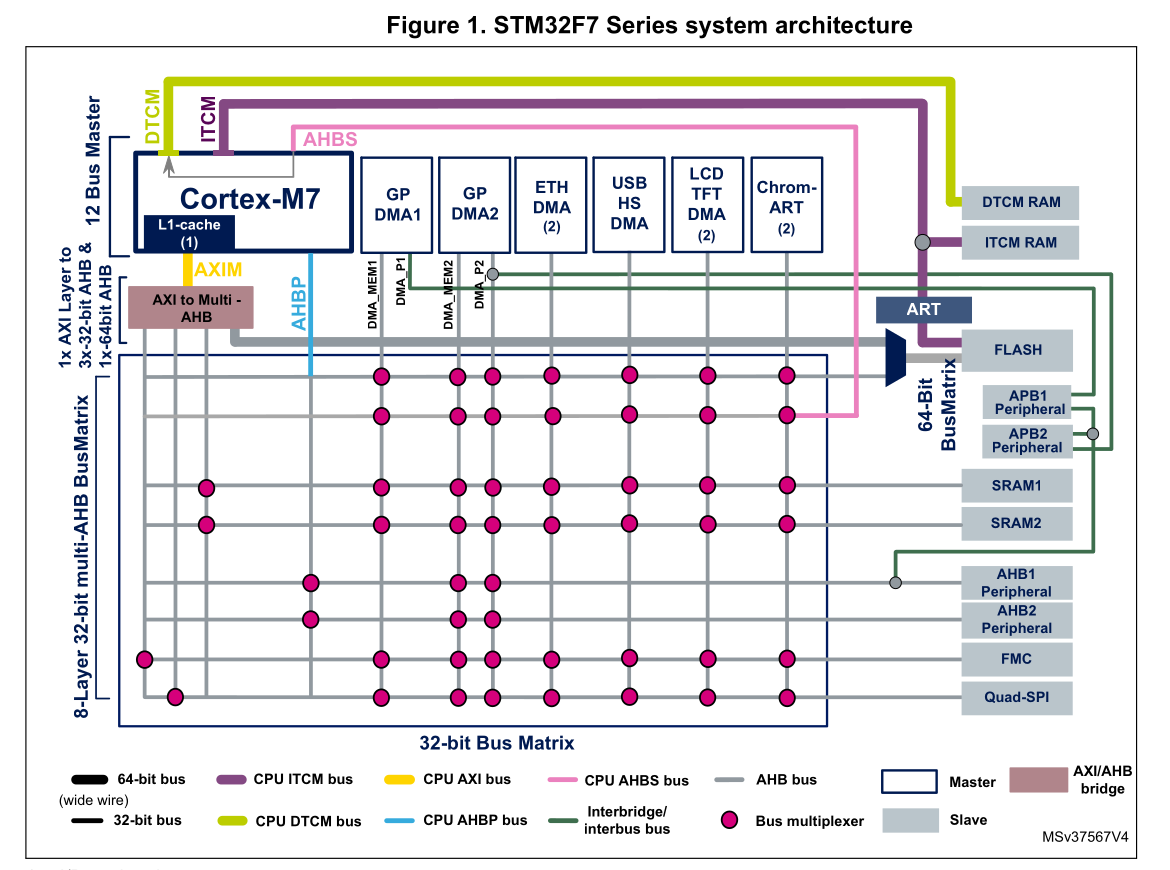
\includegraphics[width=1\textwidth]{assets/m7_system_arch}
    \caption{STM32F7 Systemarchitektur \cite[S. 9]{an4667}}
    \label{fig:m7_sys_arch}
\end{figure}

Kurz gesagt, kann jeder normale, nicht gemeinsam genutzte (non-shared)
Speicherbereich gecacht werden, sofern er über das AXI-Bus zugänglich ist
\cite[S. 4]{an4839}~\cite[S. 7]{an4667}.

Aus der Tabelle für den internen Speicher wird deutlich, dass der Flash-Speicher
ab der Adresse $0x0800,0000$ über das AHB-Bus angesprochen wird (siehe
\ref{fig:internal_mem_table}). Diese Adresse ist auch im generierten
Linker-Skript als die Standard-Flash-Adresse für die Firmware festgelegt. Daher
kann der Instruktionscache über den AXI-Bus für den Programm-Flash aktiviert
werden.

\begin{figure}[htb]
    \centering
    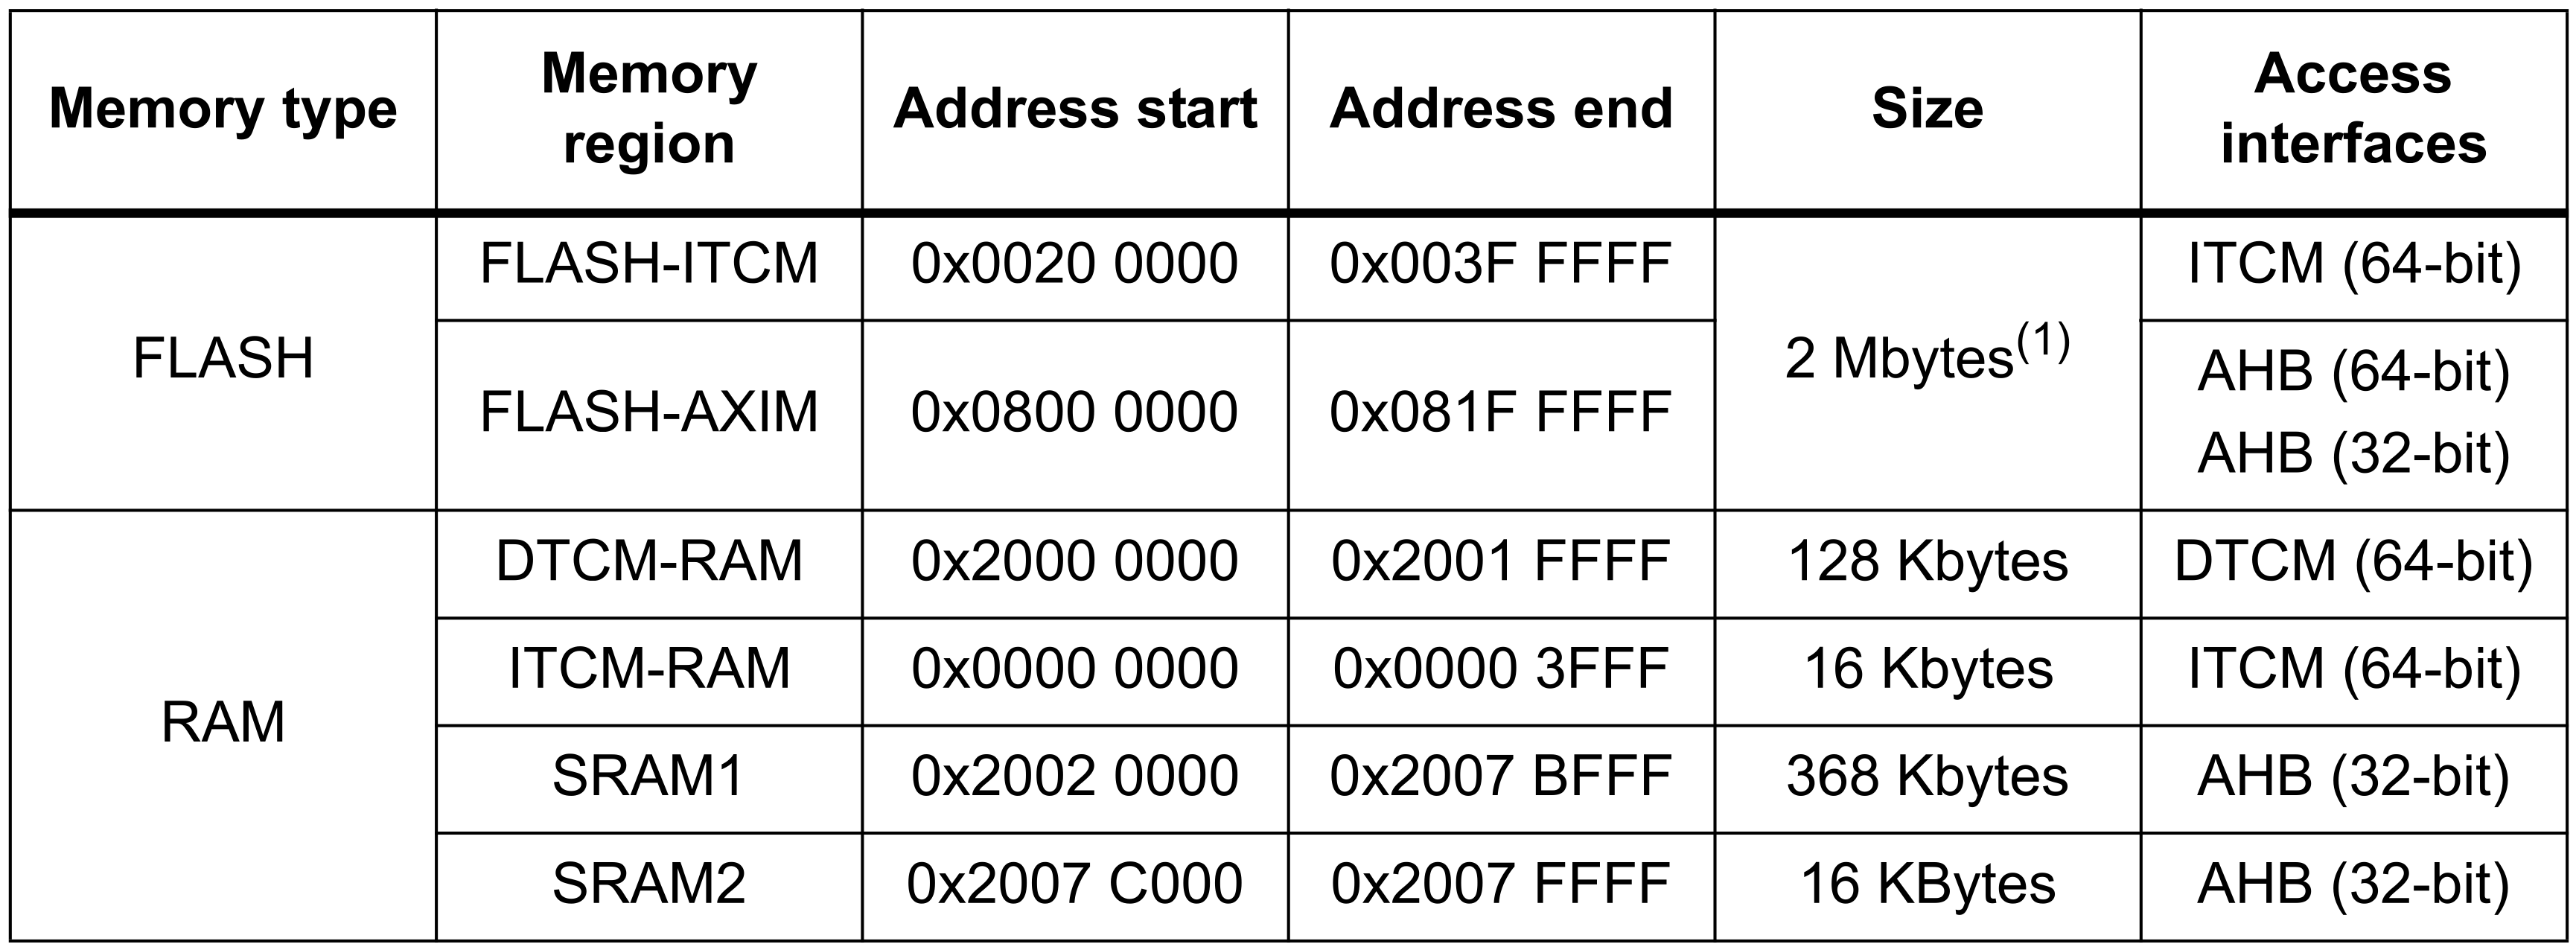
\includegraphics[width=1\textwidth]{assets/internal_mem_table}
    \caption{STM32F7 Systemarchitektur \cite[S. 14]{an4667}}
    \label{fig:internal_mem_table}
\end{figure}

\begin{code}
\begin{minted}{c}
MEMORY
{
RAM (xrw)      : ORIGIN = 0x20000000, LENGTH = 512K
FLASH (rx)      : ORIGIN = 0x8000000, LENGTH = 2048K
}
\end{minted}
    \captionof{listing}{Definition Speicherbereich im Linker-Script für STM32F7}
\end{code}

Um Caches zu nutzen, bietet die STM-\ac{HAL} dedizierte Funktionsaufrufe in der
API an \cite[S. 4]{an4839}:

\begin{code}
\begin{minted}{c}
void SCB_EnableICache(void)
void SCB_DisableICache(void)
void SCB_InvalidateICache(void)
void SCB_EnableDCache(void)
void SCB_DisableDCache(void)
void SCB_InvalidateDCache(void)
void SCB_CleanDCache(void)
void SCB_CleanInvalidateDCache(void)
\end{minted}
    \captionof{listing}{Cache-Funktionen}
\end{code}

Bei einer Cache-Clean-Operation werden modifizierte Cache-Zeilen (Dirty Cache
Lines), die durch das Programm aktualisiert wurden, zurück in den Hauptspeicher
geschrieben. Dieser Vorgang wird gelegentlich auch als „flush” bezeichnet
\cite[S. 4]{an4839}. Eine Cache-Invalidierungsoperation markiert den Inhalt des
Caches als ungültig, sodass bei einem erneuten Zugriff auf dieselben Daten der
Speicher neu ausgelesen und der Cache aktualisiert werden muss.

Allerdings kann beim Aktivieren von Caches für Speicherbereiche, die vom
DMA-Controller genutzt werden, ein Problem der Cache-Kohärenz (Cache Coherency)
entstehen, da der Prozessor in diesem Fall nicht der einzige Master ist, der auf
diese Speicherbereiche schreibt und liest. Daher sind Operationen wie
Cache-Clean und Cache-Invalidierung essentiell, um die Konsistenz zwischen Cache
und Speicher sicherzustellen.

\subsubsection{Cache-Clean bei DMA}

Damit der DMA-Controller stets auf aktuelle Daten zugreifen kann, ist eine
Cache-Clean nach jeder Datenmodifikation erforderlich. Sie stellt sicher, dass
die Daten nicht nur im Cache modifiziert, sondern auch noch zurück in den
Speicher geschrieben werden \cite[S. 6]{an4839}. Ohne diesen Schritt würden die
Änderungen nicht im SRAM widergespiegelt, und der DMA-Controller würde weiterhin
veraltete Daten verwenden.

\subsubsection{Cache-Invalidierung bei DMA}

Bei Daten, die aus Speicherbereichen gelesen werden, auf die auch der
DMA-Controller zugreift, muss zuvor eine Cache-Invalidierung erfolgen
\cite{embeddedexpert_cache}. Dies garantiert, dass die Daten immer direkt aus
dem RAM gelesen werden. Da der DMA-Controller die Daten jederzeit ändern kann,
sind die gecachten Daten per se ungültig und müssen durch eine Aktualisierung
ersetzt werden.

\subsection{Aktivierung von Instruktionscache}

TODO
